\section{Methodology}
This research involves creating a model of the appraisal process to predict the appraisal as remembered in terms of situational interdependence. The schematic representation of the prediction model is described in Figure \ref{fig:model_diagram}. The diagram illustrates Person A in a conversation, showing that the appraisal in the moment is estimated from some observable signals that indicate the appraisal. For example, Person A can be smiling (facial cue) while talking (verbal cue) and making hand gestures (behavioural cue), where each of these cues could potentially indicate a different aspect of appraisal. The modelled Person A's appraisal in the moment is the input for the predictive model, generating predicted values for appraisal as remembered. Subsequently, the outcomes are compared with actual data to test the hypotheses.
\begin{figure}
    \centering
    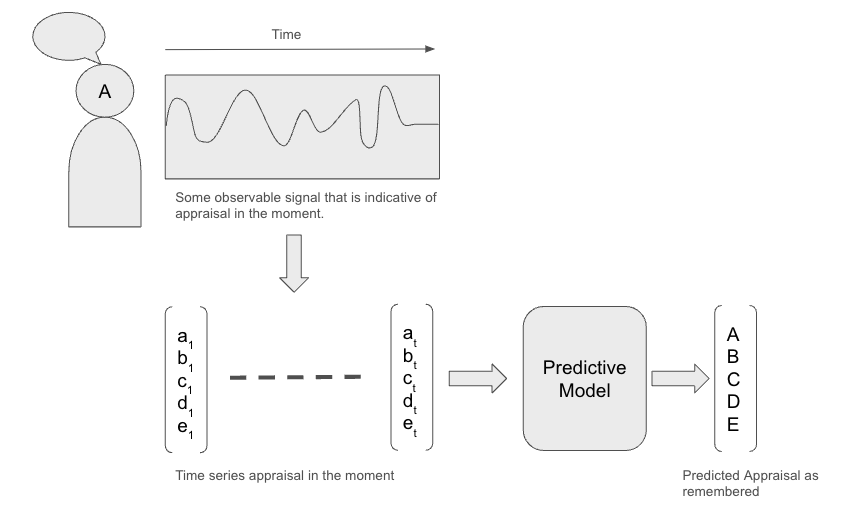
\includegraphics[width=\linewidth]{Images/schematic1.png}
    \caption{Schematic Representation of Situational Interdependence Prediction Model}
    \label{fig:model_diagram}
\end{figure}

\subsection{Dataset}
This research employs two distinct datasets: the PACO dataset \cite{matej2022designing} and the Negotiation dataset \cite{recorgnizing2021Dudzik}. Although they were collected for different purposes, both datasets provide comparable information relevant to our research aims. This includes audio-visual recordings of participants engaging in conversations from similar angles, along with post-conversation SIS measurements. In short, conversation records under the listed five contexts were present in the two datasets.

\begin{enumerate}
    \item Joint trust task setting (TRUST)
    \item Joint competence task setting (COMP)
    \item Feud Task setting (FEUD)
    \item Low conflict Negotiation setting (LConf)
    \item High conflict Negotiation setting (HConf)
\end{enumerate}

% explanation of paco
The PACO dataset \cite{matej2022designing} was initially developed to model partner selection and explore its relationship with human impressions during social interactions \cite{matej2022designing}. The dataset includes recordings of 3-minute online conversations between two individuals over three different contextual settings. The settings include performing 1) a joint trust task (TRUST), which is a cooperative decision-making task with mixed motives, 2) a joint competence task (COMP), where the outcome depends on the competence of two individuals, and 3) a Feud Task (FEUD), where facilitation of collaboration and active communication are important for the best outcome. Half of the participants were selected for performing the joint trust task and the other for the joint competence task. The feud tasks were performed by all participants. Each participant was asked to have one-on-one online video conversations for the two tasks with 3-5 other participants and to fill out a questionnaire including a 10-item version of questions from SIS after each conversation.

% Explanation of negotiation dataset
The other dataset is the Negotiation dataset \cite{recorgnizing2021Dudzik}. It contains recordings of negotiation conversations in face-to-face settings between two individuals. One of the participants was assigned to the "applicant" and the other to the "HR manager", where the latter has more power in the setting. The conversations are assigned to one of two conditions in terms of the intensity of conflict. The low conflict situation (LConf) has more options, five out of five options, which leads to a preferred outcome of both of them while the high conflict situation (HConf) has only one option and the rest leads to a consequence where one's best outcome is the other's worst outcome. Participants needed to carry out the 5-minute negotiation three times and fill out a survey that included a 10-item version of SIS, the same set of questions with the PACO, after each session. After the third session, they had to come up with an agreement and failure to do so had a consequence of either 60\%, 40\%, or 20\% of an even split.

\subsection{Modelling appraisal in the moment}
% % Valance, Arousal from non-textual verbal cue
% As mentioned in the section \ref{intro}, one of the overlapping dimensions of the appraisal process and situation perception is valance, which is the extent of how positively an individual perceives a situation. It can also be expected that the dominance, which is one of an outcome or indication of the appraisal process, could be reflective of the actual power that an individual has in a conversation, which is also one of the determinants of situational interdependence, which is found to be predictable from non-verbal cue \cite{recorgnizing2021Dudzik}. There is evidence that valance can be extracted from speech signals. In this research, a model for dimensional speech emotion recognition is going to be used \cite{wagner2023dawn} to exploit non-textual verbal cues. This model is based on pre-trained wav2vec 2.0 \cite{Baevski2020Advances}, which processes the input audio file into frozen CNN first and then the inner Transformer layer is fine-tuned to output a learned representation. It is then used to extract emotional dimensions of valance, arousal, and dominance by being trained on MSP-Podcast \cite{Lotfian2019building}. The implementation is available on Github \footnote{https://github.com/audeering/w2v2-how-to}. The limitation here is that the emotional expressions observed in the speech signal might not reflect the actual internal states or power distribution of an individual, thus here we assume that it is the case. 

% LLM are used to model appraisal in the moment in terms of SIS. 
As mentioned earlier in Section \ref{app_model}, the usage of LLM has been attempted previously in modelling emotional appraisal from textual content. This research is also going to follow this trend of using LLM to model the appraisal in the moment by looking at the textual conversation contents. Since the dimensions of the appraisal as remembered are in terms of the situational interdependence scale (SIS), the modelling of appraisal in the moment will also be in terms of the SIS. 

% The query has two types, 1) task definition 2) query
In formulating the prompt to model appraisal in the moment, we adopt a methodology similar to that of \citeauthor{feng2023affect}\cite{feng2023affect}. Their study is particularly relevant as it specifically addresses conversation settings. We incorporate two types of prompts: task definitions and queries. It's worth noting that \citeauthor{feng2023affect} also experimented with in-context learning; however, due to the absence of ground truth labels for appraisal dimensions in the moment in the datasets, we are unable to utilize this aspect in our setup. The task definition involves outlining each dimension of situational interdependence and describing the contextual setting. 

% The appraisal modelling takes place per utterance. Once it is evaluated, it is added to the conversation history for the next utterance query.
Meanwhile, the structure of the query prompt draws inspiration from \citeauthor{feng2023affect}\cite{feng2023affect}, with a focus on the process of appraisal estimation for each new utterance while maintaining the history of the conversation as context for future queries. The utterance of the conversation partner is also added to the conversation history. The example prompt is shown in Table \ref{tab:prompts}.

\begin{table}
    \centering
    \begin{tabular}{|p{3cm}|p{7cm}|} \hline
         Prompt type & Prompt template \\ \hhline{|==|}
         Task Definition & Consider the following list of concepts, called "Situational Interdependence" : [Mutual Dependence : (definition), Conflict of Interest : (definition), ...]\\ \hline
         Query & Given the dialogue history between PersonA and PersonB : [PersonA: ..., PersonB: ..., ...], what is the "Situational Interdependence" in the next utterance of PersonA "..."? \\ \hline
    \end{tabular}
    \caption{Templates of prompts for modelling appraisal in the moment. }
    \label{tab:prompts}
\end{table}

% The formulation of the prompt to model the appraisal dimensions using the Likert scale is inspired by several research \cite{feng2023affect, zhan-etal-2023-evaluating}. Out of the relevant papers which are found so far \cite{broekens2023fine, tak2023gpt, yongsatianchot2023investigating, zhan-etal-2023-evaluating}, \citeauthor{feng2023affect}'s experiment \cite{feng2023affect} seems to the closest settings to our experiment. They processed each utterance to identify emotions from a set of emotional labels within a conversational context, providing valuable inspiration for our study. 

\subsection{Predictive model}
The predictive model takes the time-variant appraisal in the moment in terms of situational interdependence as its input and the predicted values of appraisal as remembered in terms of situational interdependence as its output. To maintain the time-variant nature of appraisal for prediction, we utilize the Long Short-Term Memory network (LSTM). The LSTM's ability to capture long dependencies over time is well-suited for our task. To address RQ1, all instances of data are utilized, whereas for RQ2, a new network is trained for each contextual setting.

% Maybe Randomforest too but need to find papers
% Maybe Reinforcement learning too but need to find papers


% https://inria.github.io/scikit-learn-mooc/python_scripts/dev_features_importance.html

% Some ideas for the models
% Tim's paper